\documentclass[journal,12pt,twocolumn]{IEEEtran}

\usepackage{setspace}
\usepackage{gensymb}
\singlespacing
\usepackage[cmex10]{amsmath}

\usepackage{amsthm}

\usepackage{mathrsfs}
\usepackage{txfonts}
\usepackage{stfloats}
\usepackage{bm}
\usepackage{cite}
\usepackage{cases}
\usepackage{subfig}

\usepackage{longtable}
\usepackage{multirow}

\usepackage{enumitem}
\usepackage{mathtools}
\usepackage{steinmetz}
\usepackage{tikz}
\usepackage{circuitikz}
\usepackage{verbatim}
\usepackage{tfrupee}
\usepackage[breaklinks=true]{hyperref}
\usepackage{graphicx}
\usepackage{tkz-euclide}

\usetikzlibrary{calc,math}
\usepackage{listings}
    \usepackage{color}                                            %%
    \usepackage{array}                                            %%
    \usepackage{longtable}                                        %%
    \usepackage{calc}                                             %%
    \usepackage{multirow}                                         %%
    \usepackage{hhline}                                           %%
    \usepackage{ifthen}                                           %%
    \usepackage{lscape}     
\usepackage{multicol}
\usepackage{chngcntr}

\DeclareMathOperator*{\Res}{Res}

\renewcommand\thesection{\arabic{section}}
\renewcommand\thesubsection{\thesection.\arabic{subsection}}
\renewcommand\thesubsubsection{\thesubsection.\arabic{subsubsection}}

\renewcommand\thesectiondis{\arabic{section}}
\renewcommand\thesubsectiondis{\thesectiondis.\arabic{subsection}}
\renewcommand\thesubsubsectiondis{\thesubsectiondis.\arabic{subsubsection}}


\hyphenation{op-tical net-works semi-conduc-tor}
\def\inputGnumericTable{}                                 %%

\lstset{
%language=C,
frame=single, 
breaklines=true,
columns=fullflexible
}
\begin{document}


\newtheorem{theorem}{Theorem}[section]
\newtheorem{problem}{Problem}
\newtheorem{proposition}{Proposition}[section]
\newtheorem{lemma}{Lemma}[section]
\newtheorem{corollary}[theorem]{Corollary}
\newtheorem{example}{Example}[section]
\newtheorem{definition}[problem]{Definition}

\newcommand{\BEQA}{\begin{eqnarray}}
\newcommand{\EEQA}{\end{eqnarray}}
\newcommand{\define}{\stackrel{\triangle}{=}}
\bibliographystyle{IEEEtran}
\raggedbottom
\setlength{\parindent}{0pt}
\providecommand{\mbf}{\mathbf}
\providecommand{\pr}[1]{\ensuremath{\Pr\left(#1\right)}}
\providecommand{\qfunc}[1]{\ensuremath{Q\left(#1\right)}}
\providecommand{\sbrak}[1]{\ensuremath{{}\left[#1\right]}}
\providecommand{\lsbrak}[1]{\ensuremath{{}\left[#1\right.}}
\providecommand{\rsbrak}[1]{\ensuremath{{}\left.#1\right]}}
\providecommand{\brak}[1]{\ensuremath{\left(#1\right)}}
\providecommand{\lbrak}[1]{\ensuremath{\left(#1\right.}}
\providecommand{\rbrak}[1]{\ensuremath{\left.#1\right)}}
\providecommand{\cbrak}[1]{\ensuremath{\left\{#1\right\}}}
\providecommand{\lcbrak}[1]{\ensuremath{\left\{#1\right.}}
\providecommand{\rcbrak}[1]{\ensuremath{\left.#1\right\}}}
\theoremstyle{remark}
\newtheorem{rem}{Remark}
\newcommand{\sgn}{\mathop{\mathrm{sgn}}}
\providecommand{\abs}[1]{\left\vert#1\right\vert}
\providecommand{\res}[1]{\Res\displaylimits_{#1}} 
\providecommand{\norm}[1]{\left\lVert#1\right\rVert}
\providecommand{\norm}[1]{\lVert#1\rVert}
\providecommand{\mtx}[1]{\mathbf{#1}}
\providecommand{\mean}[1]{E\left[ #1 \right]}
\providecommand{\fourier}{\overset{\mathcal{F}}{ \rightleftharpoons}}
%\providecommand{\hilbert}{\overset{\mathcal{H}}{ \rightleftharpoons}}
\providecommand{\system}{\overset{\mathcal{H}}{ \longleftrightarrow}}
	%\newcommand{\solution}[2]{\textbf{Solution:}{#1}}
\newcommand{\solution}{\noindent \textbf{Solution: }}
\newcommand{\cosec}{\,\text{cosec}\,}
\providecommand{\dec}[2]{\ensuremath{\overset{#1}{\underset{#2}{\gtrless}}}}
\newcommand{\myvec}[1]{\ensuremath{\begin{pmatrix}#1\end{pmatrix}}}
\newcommand{\mydet}[1]{\ensuremath{\begin{vmatrix}#1\end{vmatrix}}}
\numberwithin{equation}{subsection}
\makeatletter
\@addtoreset{figure}{problem}
\makeatother
\let\StandardTheFigure\thefigure
\let\vec\mathbf
\renewcommand{\thefigure}{\theproblem}
\def\putbox#1#2#3{\makebox[0in][l]{\makebox[#1][l]{}\raisebox{\baselineskip}[0in][0in]{\raisebox{#2}[0in][0in]{#3}}}}
     \def\rightbox#1{\makebox[0in][r]{#1}}
     \def\centbox#1{\makebox[0in]{#1}}
     \def\topbox#1{\raisebox{-\baselineskip}[0in][0in]{#1}}
     \def\midbox#1{\raisebox{-0.5\baselineskip}[0in][0in]{#1}}
\vspace{3cm}
\title{Assignment 1}
\author{AAYUSH GOYAL - EE18BTECH11001}
\maketitle
\newpage
\bigskip
\renewcommand{\thefigure}{\theenumi}
\renewcommand{\thetable}{\theenumi}
Download all python codes from 
\begin{lstlisting}
https://github.com/aayush2710/EE3025_A1/codes
\end{lstlisting}
%
and latex-tikz codes from 
%
\begin{lstlisting}
https://github.com/aayush2710/EE3025_A1
\end{lstlisting}
\section{Problem}
(5.3) The system h(n) is said to be stable if \\
\begin{align}
\sum_{n=-\infty}^{\infty} \abs{h(n)} < \infty
\end{align}
Is the system defined by (3.2) stable for impulse response in (5.1)?
\section{Solution}
\textbf{BIBO Stability} : For a system to be stable, bounded input should result in bounded output.


If
\begin{align}
\sum_{n=-\infty}^{\infty} \abs{x(n)} < \infty
\end{align}
Then
\begin{align}
\sum_{n=-\infty}^{\infty} \abs{y(n)} < \infty
\end{align}

Let us assume,
\begin{align}
\sum_{n=-\infty}^{\infty} \abs{x(n)} < B_{x} < \infty \\
\abs{y(n)} = \abs{\sum_{-\infty}^{\infty}h(k)x(n-k)} \\
\abs{y(n)} \leq \sum_{-\infty}^{\infty}\abs{h(k)}\sum_{-\infty}^{\infty}\abs{x(n-k)}\\
\abs{y(n)} \leq B_x\sum_{-\infty}^{\infty}\abs{h(k)}\\
\implies \sum_{n=-\infty}^{\infty} \abs{y(n)} < B_{y} < \infty
\end{align}
only when h(n) is bounded i.e
\begin{align}
\sum_{n=-\infty}^{\infty} \abs{h(n)}  &< \infty \\
\sum_{n=-\infty}^{\infty}\abs{h(n)}\abs{z^{-n}}_{\abs{z}=1}&<\infty\\
\sum_{n=-\infty}^{\infty}\abs{h(n)z^{-n}}_{\abs{z}=1}&<\infty \\
\sum_{n=-\infty}^{\infty}\abs{h(n)z^{-n}}_{\abs{z}=1}&<\abs{\sum_{n=-\infty}^{\infty}h(n)z^{-n}}_{\abs{z}=1} \\
\implies \abs{H(z)}_{\abs{z}=1}&<\infty
\end{align}

\textbf{Conclusion : For a stable system, ROC of the system must include unit circle}

Given the following difference equation

\begin{align}
y(n) + \frac{1}{2} y(n-1) = x(n) + x(n-2)
\end{align}

Applying Z-Transform

\begin{align}
Y(z) + \frac{1}{2} z^{-1}Y(z) &= X(z) + z^{-2}X(z) \\
H(z) &= \frac{Y(z)}{X(z)} = \dfrac{1 + z^{-2}}{1 + \frac{1}{2} z^{-1}} \\
H(z) &= \frac{2(z^{2} +1)}{z(2z+1)} \\
\implies Poles &= 0 , -\frac{1}{2}
\end{align}

ROC of h(n) (Right sided system) lies outside the outermost pole ($\frac{1}{2}$)

H(z) is plotted in z-plane using python via the following script
\\
\begin{lstlisting}
https://github.com/aayush2710/EE3025_A1/codes/zplot.py
\end{lstlisting}

Observe that in figure \ref{Z_plane analysis}, $\abs{z} = 1$ clearly lies inside ROC.

$\implies$ System is stable.


\begin{figure}[h!]
    \centering
    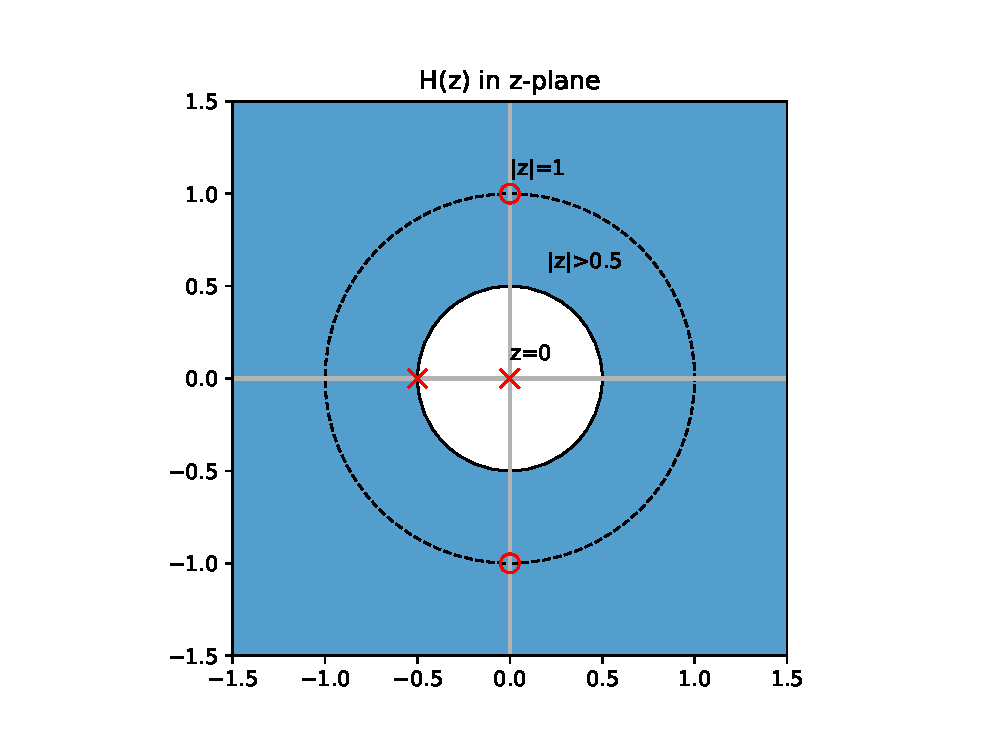
\includegraphics[width=10cm]{./figs/zplane.eps}
    \caption{H(z) in z-plane}
    \label{Z_plane analysis}
\end{figure}

\section{Verification}

Let us assume a bounded input

\begin{align}
    x(n) = \cbrak{\underset{\uparrow}{1},2,3,4,2,1}\\
    y(n)+\frac{1}{2}y(n-1) = x(n)+x(n-2)
\end{align}

\begin{figure}[h!]
    \centering
    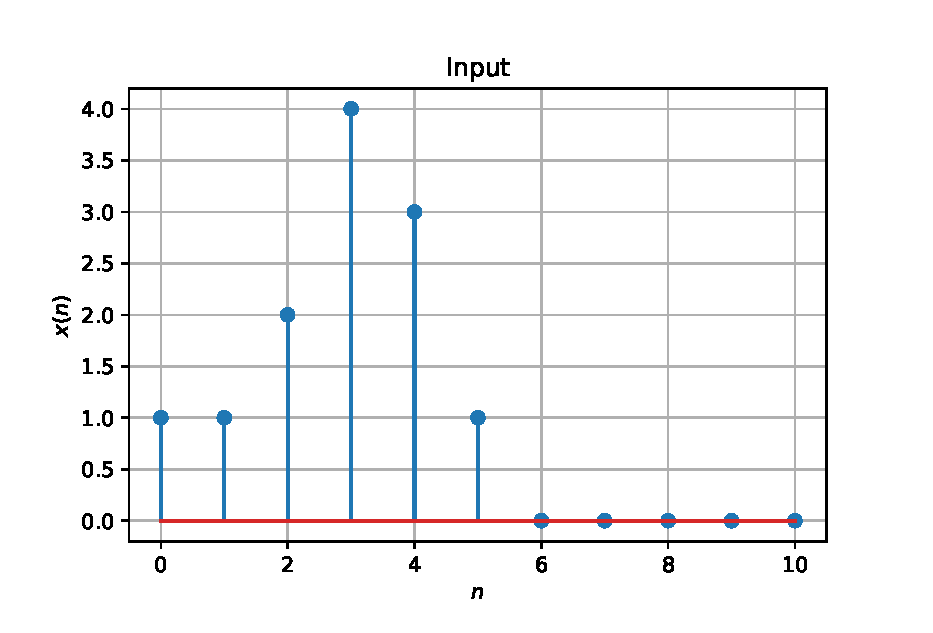
\includegraphics[width=9cm]{./figs/fig_x.eps}
    \caption{Input x(n)}
    \label{x(n)}
\end{figure}

Clearly x(n) is absolutely summable

We can calculate y(n) using the difference equation

Use the following code to plot Input, Output and Impulse Response
\\
\begin{lstlisting}
https://github.com/aayush2710/EE3025_A1/codes/xyplot.py
\end{lstlisting}

\begin{figure}[h!]
    \centering
    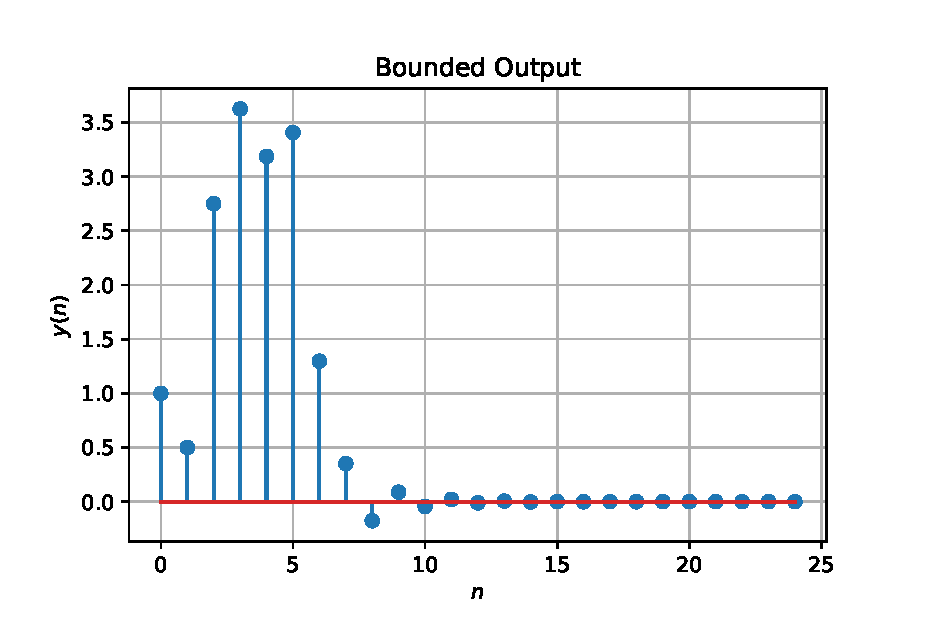
\includegraphics[width=10cm]{./figs/fig_y.eps}
    \caption{Output y(n)}
    \label{y(n)}
\end{figure}

Clearly y(n) is absolutely summable as shown in figure \ref{y(n)}. Hence Bounded Input results in Bounded Output. This verifies the above solution.


\begin{figure}[h!]
    \centering
    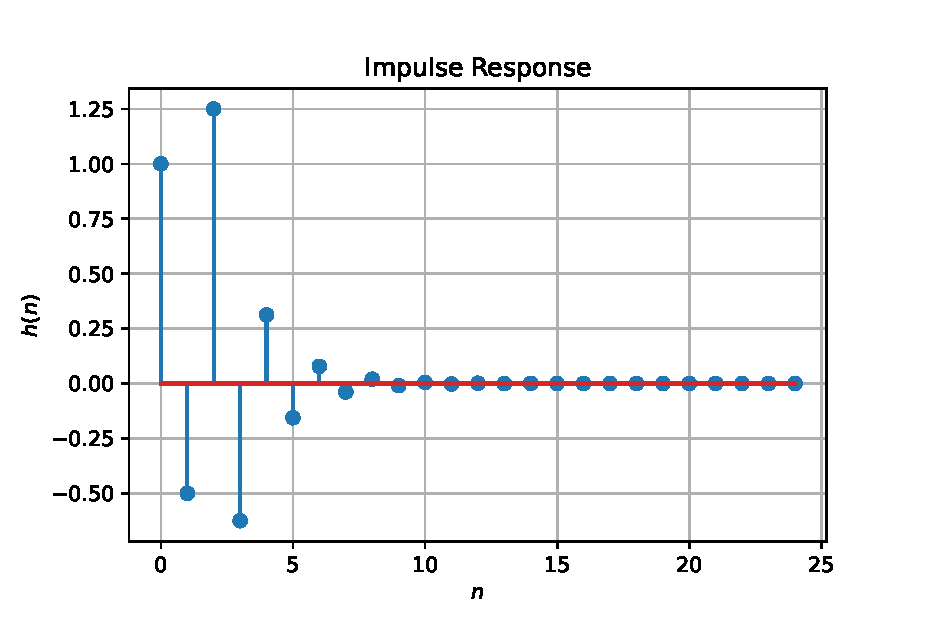
\includegraphics[width=10cm]{./figs/fig_h.eps}
    \caption{Impulse Response h(n)}
    \label{h(n)}
\end{figure}

Further Impulse Response $h(n)$ of our system is also bounded as shown in figure \ref{h(n)}.
\end{document}